\documentclass[handout]{beamer}
\usepackage[utf8]{inputenc}
\usepackage{graphics}
\mode<presentation> {
\usetheme{unc}}
\setbeamertemplate{navigation symbols}{} % To remove the navigation symbols from the bottom of all slides uncomment this line

\usepackage{graphicx} % Allows including images
\usepackage{booktabs} % Allows the use of \toprule, \midrule and \bottomrule in tables


\usepackage{hyperref}
\hypersetup{linkcolor=blue,colorlinks=true}


% Remove symbols
\beamertemplatenavigationsymbolsempty


%\usetheme{default}

\usefonttheme{serif}

%----------------------------------------------------------------------------------------
%	TITLE PAGE
%----------------------------------------------------------------------------------------


\title[Alliances and Collective Security]{\LARGE{Alliances and Collective Security}}
\author[POLI 150]{Steven Saroka}
\institute{POLI 150}
\date{8 February 2024}


\begin{document}

\begin{frame}
\titlepage % Print the title page as the first slide
\end{frame}


%----------------------------------------------------------------------------------------
%	PRESENTATION SLIDES
%----------------------------------------------------------------------------------------

%% Slide outline

\begin{frame} 
	\frametitle{\LARGE{Reminders}}
	\begin{itemize}
		\Large{
			\item Prompt 5 due tonight.

		}
	\end{itemize}
\end{frame}

\begin{frame} 
	\frametitle{\LARGE{Today's Class}}
	\begin{itemize}
		\Large{
			\item Alliances and Crisis Bargaining
			\\~\\ 
			\item NATO
			\\~\\
			\item UN and Collective Security
			\\~\\
			\item UNC Conflict Research
		}
	\end{itemize}
\end{frame}

\begin{frame} 
	\frametitle{\LARGE{Central Questions}}
	\centering
	\Large{How do international institutions influence interstate war? What conflict research has been published recently at UNC?}
\end{frame}

\begin{frame} 
	\frametitle{\LARGE{Key Terms}}
	\begin{itemize}
		\item International Institutions
		\item Alliances 
		\item NATO
		\item Collective Defense
		\item Collective Security
		\item UN
	\end{itemize}
\end{frame}

\begin{frame} 
	\frametitle{\LARGE{Anarchy and International Institutions}}
	\begin{itemize}
		\item The international system is anarchic. \pause
		\item In spite of this, we frequently observe cooperation between states on a variety of issues: security, economic, environmental, etc.
		\item This cooperation is frequently facilitated by \textbf{International Institutions}: a common set of rules shared among states that structure their interactions in specific ways. \pause
		\item This lecture focuses on the impact of these institutions on interstate war.
	\end{itemize}
\end{frame}

\begin{frame} 
\frametitle{\LARGE{Alliances}}
	\begin{itemize}
		\item \textbf{Alliance}: institution that helps member states cooperate on their security policy and in the event of a war. \pause 
		\item Alliances include states with compatible security interests. \pause
		\item They frequently describe standards about how states will behave if conflict arises between a non-member and member(s). \pause
		\item Ultimately, alliances form out of common security interests.
	\end{itemize}
\end{frame}


\begin{frame} 
	\frametitle{\LARGE{Alliance Subtypes}}
Alliances can vary by whether they are...
	\begin{itemize}
		\item \textbf{Bilateral vs. Multilateral}: between two or more than two states. \pause
		\item\textbf{Offensive vs. Defensive}: states cooperate to attack another vs. states defend each other in case of attack. \pause
		\item \textbf{Asymmetric vs. Symmetric}: between states with a power disparity or states with relatively equal power.
	\end{itemize}
\end{frame}

\begin{frame} 
	\frametitle{\LARGE{Alliance Subtype Examples}}
	\begin{itemize}
		\item NATO: multilateral, asymmetric, defensive. \pause
		\item US and South Korea: bilateral, asymmetric, defensive. \pause
		\item Molotov-Ribbentrop Pact: bilateral, symmetric, offensive.
	\end{itemize}
\end{frame}

\begin{frame} 
\frametitle{\LARGE{Why Enter Alliances?}}
	\begin{itemize}
		\item Why do states form them? 
		\item We've said they form due to common security interests, but what does that mean? \pause 
		\item Most commonly, answers appeal to the ``balance of power:" When two states fear the rise of a threatening state, banding together may allow them collectively to still be stronger than that other state.
	\end{itemize}
\end{frame}

\begin{frame} 
	\frametitle{\LARGE{Why Enter Alliances?}}
Alliance motives can also vary by a state's power or position in the international system.
	\begin{itemize}
		\item Weak state may gain protection from powerful rivals. \pause
		\item Strong state can signal its resolve to defend a weaker but strategically important state. \pause
		\item States can combine resources to allow for more effective defense. \pause
		\item Can subdue conflicts (for example, Greece and Turkey in NATO). \pause
		\item Can formalize a sphere of influence (for example, the Warsaw Pact). 		
	\end{itemize}
\end{frame}

\begin{frame} 
	\frametitle{\LARGE{Alliances and the Bargaining Model}}
	\begin{itemize}
		\item The impact of an alliance can be felt at numerous points in the bargaining model. \pause
		\item By working together in a conflict, alliances may change the location of the war outcome $x$. \pause
		\item Additionally, by working together, they may also decrease the costs $c$ for the allies or increase the costs $c$ for the opposing side.		
	\end{itemize}
\end{frame}

\begin{frame} 
	\frametitle{\LARGE{Bargaining in War}}
	\begin{figure}[ht!]
		\centering
		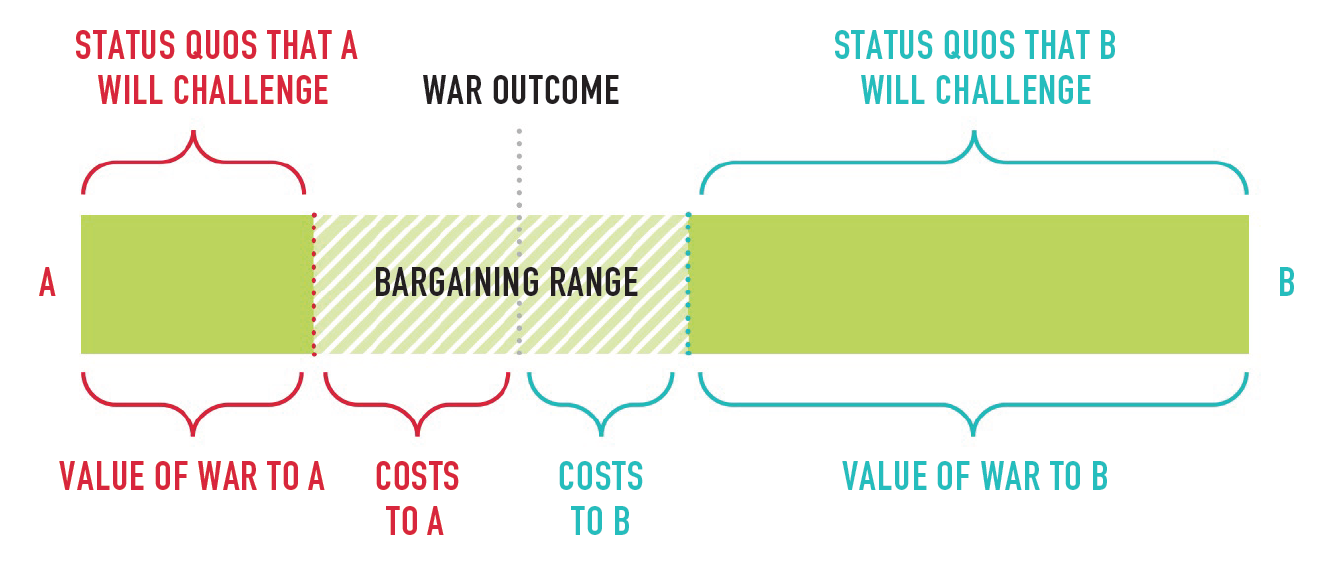
\includegraphics[width=\textwidth,height=0.8\textheight,keepaspectratio]{./nonally_bargain.png}
	\end{figure}
\end{frame}

\begin{frame} 
	\frametitle{\LARGE{Bargaining in War with an Ally}}
	\begin{figure}[ht!]
		\centering
		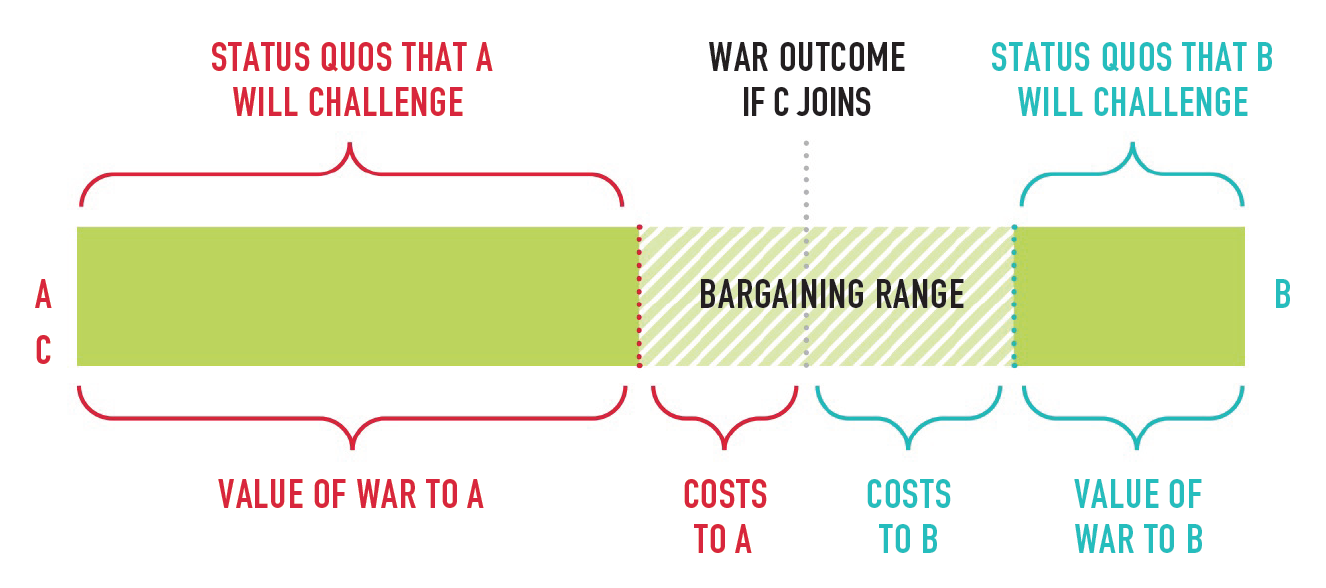
\includegraphics[width=\textwidth,height=0.8\textheight,keepaspectratio]{./ally_bargain.png}
	\end{figure}
\end{frame}

\begin{frame} 
\frametitle{\LARGE{Bargaining and Alliances}}
Alliances impact the bargaining range through all of the following mechanisms:
	\begin{itemize}
		\item Shifting the expected outcome of war in favor of the allies. \pause 
		\item Increasing the opponent's costs of war. \pause
		\item Sharing the costs of war between allies, decreasing them.
	\end{itemize}
\end{frame}



\begin{frame} 
\frametitle{\LARGE{Alliance Information Problems}}
	\begin{itemize}
		\item Thus far, we have assumed both sides believe that an ally will fight if necessary. \pause
		\item \textbf{This implies that alliances should reduce the probability of war.} \pause
		\item Why? A potential foe should look at the alliance and conclude that the costs of war will certainly be higher, while the chances of victory will be lower. \pause
		\item But, in the real world, do states always have complete information about alliances? \pause \textbf{No}. 
	\end{itemize}
\end{frame}

\begin{frame} 
	\frametitle{\LARGE{Allies and Incomplete Information}}
	\begin{itemize}
		\item Alliances fundamentally exist in a world of incomplete information. \pause
		\item States never know, until the war actually starts, whether allies will actually join the fighting. \pause
		\item However, in any alliance, the allies have incentives to misrepresent the state of the alliance: even if one side doubts that its allies are trustworthy, it will represent them as such to a potential adversary. \pause
		\item Why might an ally fail to honor its commitments? War is costly and victory is never certain. \pause
		\item Any potential adversary knows this, and thus may doubt the sincerity of any alliance claims.
		\item \textbf{Incentives to misrepresent abound here.}
	\end{itemize}
\end{frame}

\begin{frame} 
	\frametitle{\LARGE{Allies and Incomplete Information}}
This implies that an \textit{effective} alliance must do two things to deter conflict:
\begin{enumerate}
	\item Increase the chance that allies will fight together above what it would be without an alliance. \pause 
	\item Make opponents more certain that the allies will fight together than they would be without an alliance.
\end{enumerate}
How can alliances do this? \textbf{Put differently, how can alliances become credible?}
\end{frame}

\begin{frame} 
	\frametitle{\LARGE{Signaling Credibility}}
How can alliances become credible?
	\begin{itemize}
		\item Stationing troops together and engaging in joint exercises, increasing combat effectiveness. \pause  
		\item Increase costs of abandonment: tying interests together or bringing in reputation costs. \pause 
	\end{itemize}
Alliance credibility shares substantial similarities with solutions to incomplete information in the bargaining model, especially strategies of tying hands.	
\end{frame}

%pic from CBR's slides
\begin{frame} 
	\frametitle{\LARGE{Joint Military Exercises}}
	\begin{figure}[ht!]
		\centering
		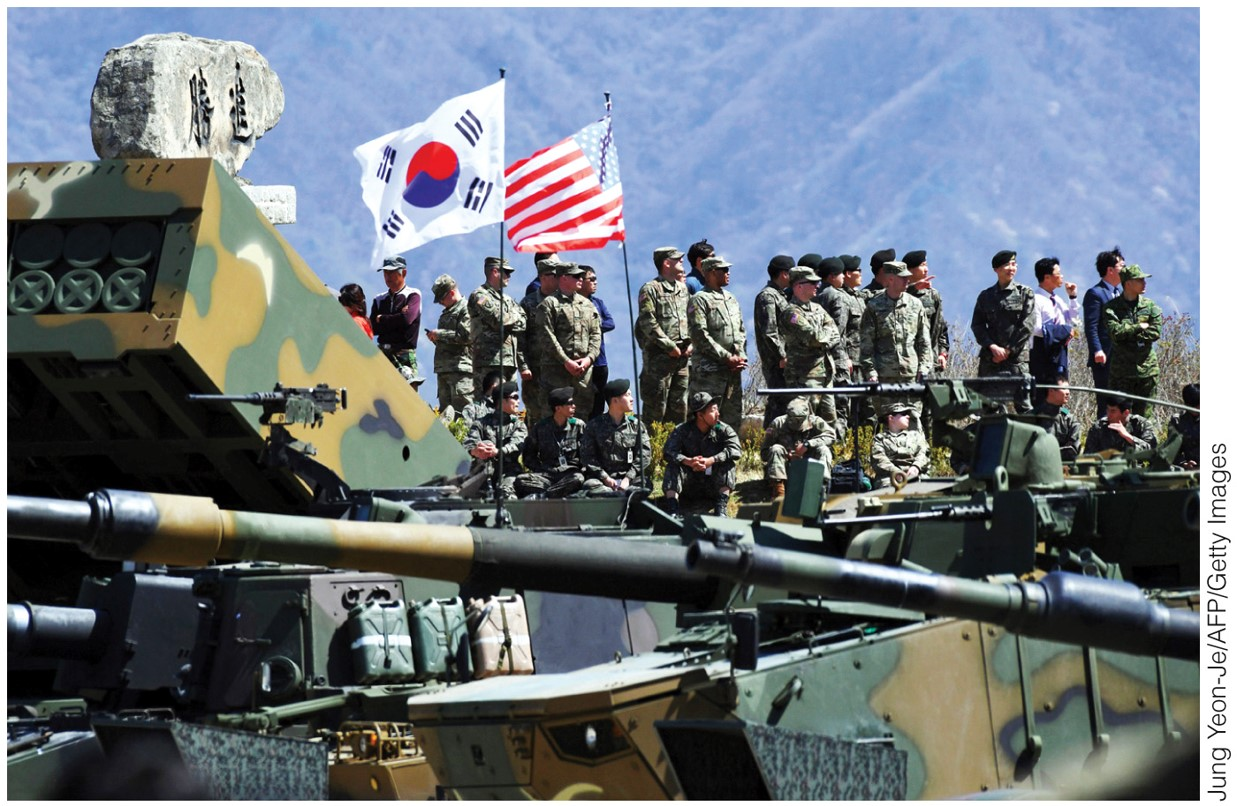
\includegraphics[width=\textwidth,height=\textheight,keepaspectratio]{USandSKjoint.jpg}
	\end{figure}
\end{frame}

\begin{frame} 
	\frametitle{\LARGE{Example: US and South Korea}}
	\begin{itemize}
		\item Approximately 28,000 US troops stationed in South Korea. \pause  
		\item Frequent military exercises involving these troops and their South Korean counterparts. \pause 
		\item These exercises make coordination and cooperation easier, decreasing costs if a war occurs, while also serving as a tying hands strategy. How? \pause
		\item If North Korea ever invades South Korea, they will likely be forced into attacking US troops, which would certainly bring the US into the war.
	\end{itemize}
\end{frame}

\begin{frame} 
	\frametitle{\LARGE{Too Much of a Good Thing?}}
		\begin{itemize}
			\item Is it possible for alliances to be detrimental to peace? \pause
			\item \textbf{Moral hazard}: Expected alliance support increases the power of states, who may make greater demands during crisis bargaining due to this anticipated support, potentially shrinking the bargaining range. \pause
			\item \textbf{Entrapment}: the risk of being dragged into an opportunistic war by an ally. \pause  
			\item Alliance treaties can try to address this via purposefully vague language.
		\end{itemize}
\end{frame}

\begin{frame} 
	\frametitle{\LARGE{Alliance Outcomes}}
	\begin{itemize}
		\item Despite incentives to misrepresent incomplete information, and the costs of war, alliance obligations are fulfilled about 70\% of the time. \pause
		\item That said, do they actually prevent conflict? \pause
		\item Example 1:  WWI and WWII
		\begin{itemize}
			\item Presence of dense set of alliances meant that any local conflict could suddenly draw in many unrelated states.
		\end{itemize}
		\item Example 2:  Cold War
		\begin{itemize}
			\item Despite the world again being aligned into two competing camps (NATO and Warsaw Pact), we did not see any direct conflict between the major powers.
		\end{itemize}
		\item The verdict: sometimes, if the alliances aren't multipolar, they can prevent conflict.
	\end{itemize}
\end{frame}

\begin{frame} 
	\frametitle{\LARGE{Alliances: NATO}}
	\begin{itemize}
		\item In the American context, NATO is the most obvious (but not only) alliance the US has. \pause
		\item \textbf{NATO}: North Atlantic Treaty Organization. A multilateral defensive alliance formed by the US post-WWII. \pause
		\begin{itemize}
			\item Warsaw Pact formed by the USSR to balance against NATO itself. \pause
		\end{itemize}
		\item Original purpose: containment of the Soviet Union. \pause
		\item Currently at 31 members. (Newest member: Finland.)
	\end{itemize}
\end{frame}

%image from https://www.statista.com/chart/26674/european-countries-by-year-of-joining-nato/
\begin{frame} 
	\frametitle{\LARGE{NATO Members and Evolution}}
	\begin{figure}[ht!]
		\centering
		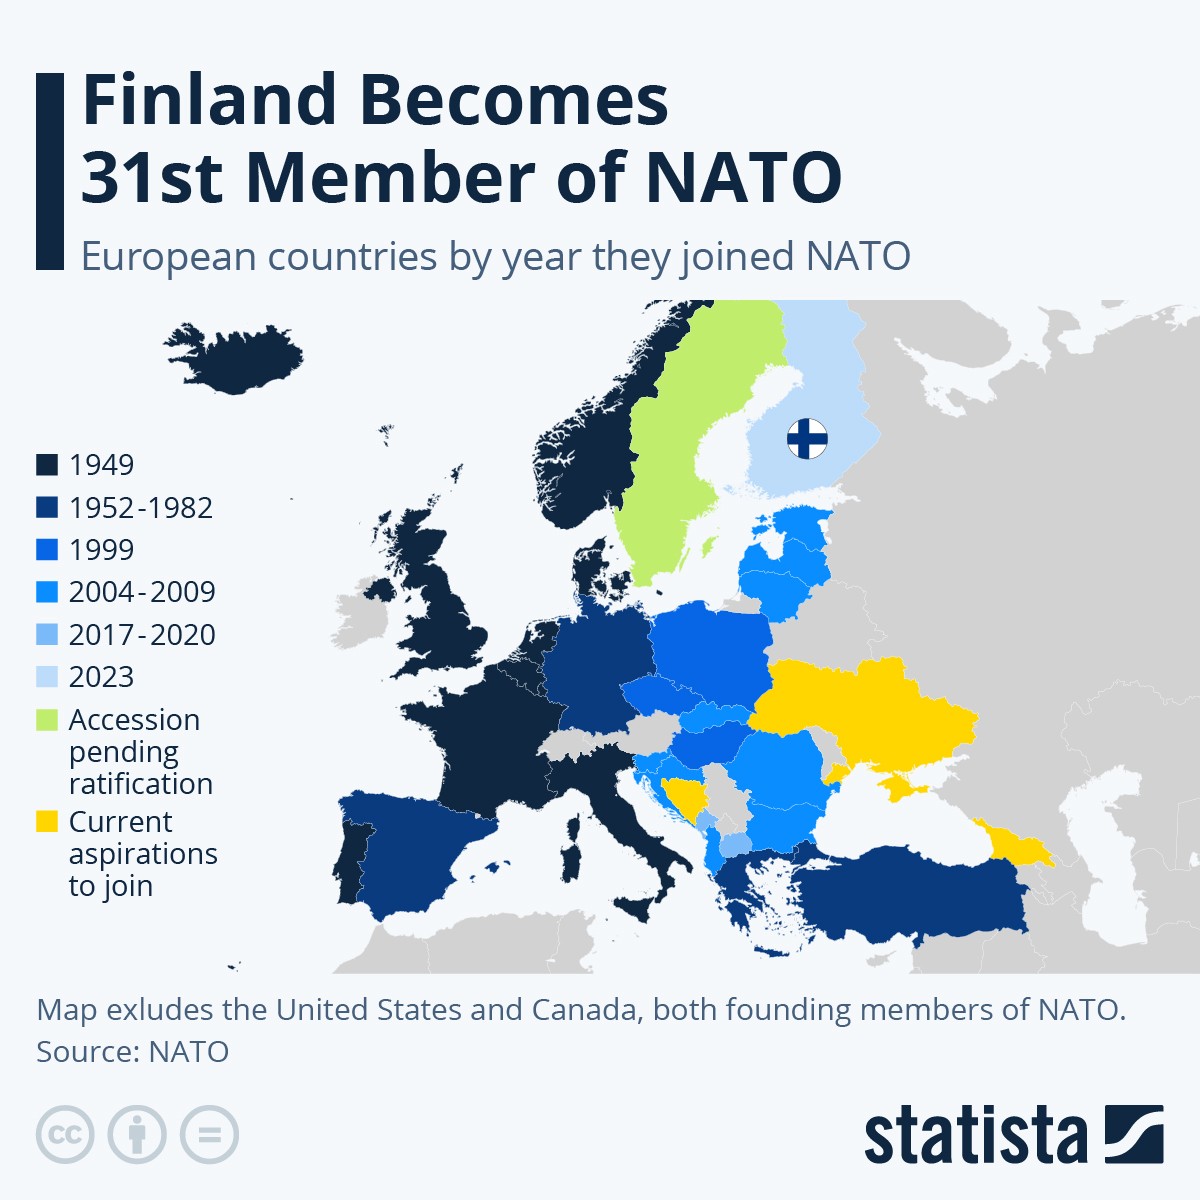
\includegraphics[width=\textwidth,height=\textheight, keepaspectratio]{NATO2023.jpeg}
	\end{figure}
\end{frame}

\begin{frame} 
\frametitle{\LARGE{NATO and Article 5}}
	\begin{itemize}
		\item Article 5 of the NATO charter is the \textbf{collective defense} provision. \pause
		\item Article 5 states that all signatories are to treat an attack against one ally as an attack against all allies. \pause 
		\item Key deterrent of Soviet aggression and a driver of peace during the Cold War.
	\end{itemize}
\end{frame}

\begin{frame} 
\frametitle{\LARGE{NATO Post-Cold War}}
	\begin{itemize}
		\item After the Cold War, analysts thought NATO would crumble like the Warsaw Pact, due to a lack of purpose. \pause 
		\item However, NATO has intervened in Kosovo, Afghanistan, and Libya. Its mission has shifted towards one general security cooperation. \pause
		\item NATO membership has continued to grow. \pause
		\item NATO expansion has incorporated 10 former members of the Warsaw Pact. \pause
	\end{itemize}
\end{frame}

\begin{frame} 
	\frametitle{\LARGE{NATO Post-Cold War}}
	\begin{itemize}
		\item US Presidents have, historically, emphasized the importance of NATO and America's commitment to the alliance. \pause
		\item Famously, Trump declined to explicitly endorse Article 5 at a NATO summit in 2017. \pause
		\begin{itemize}
			\item \textbf{What does this imply for the alliance's credibility?} \pause
		\end{itemize}
		\item Biden's tenure has been a return to the status quo, with recent NATO growth spurred by Russian aggression.
	\end{itemize}
\end{frame}
	
\begin{frame} 
	\frametitle{\LARGE{Collective Security: the United Nations}}
	\begin{figure}[ht!]
		\centering
		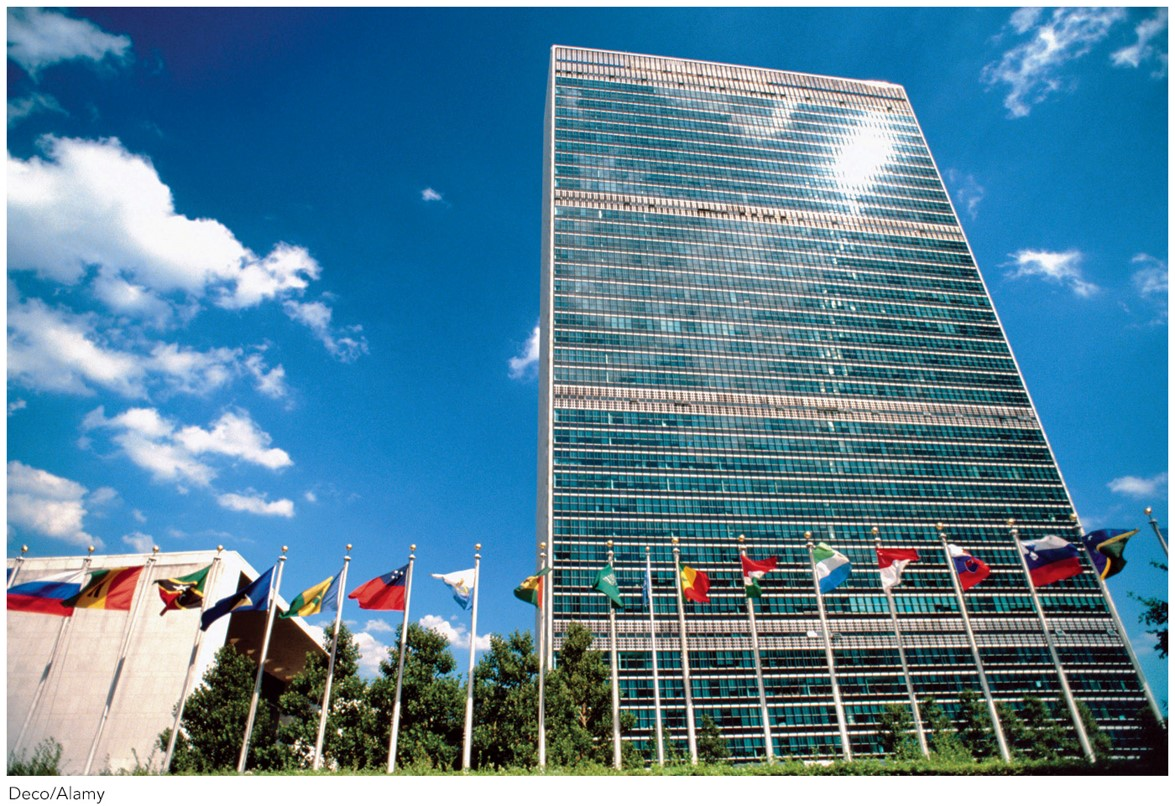
\includegraphics[width=\textwidth,height=\textheight,keepaspectratio]{UNhq.jpg}
	\end{figure}
\end{frame}	

\begin{frame} 
	\frametitle{\LARGE{Collective Security Organizations}}
		\begin{itemize}
			\item \textbf{Collective security organizations}: institution(s) formed around an interest (presumably) common to all states - global peace.  \pause 
			\item In a CSO, members pledge to aid any state that is attacked by any other state, treating an attack against one state as an attack on all. \pause
			\item In theory, this means that any potential aggressor should be deterred by the collective might of all other countries. \pause
			\item This should then incentivize peaceful negotiation rather than war. \pause
			\item Example: the UN.
		\end{itemize}
\end{frame}


\begin{frame} 
	\frametitle{\LARGE{CSOs vs. Alliances}}
This just sounds like a very large alliance. What's the difference?
	\begin{itemize}
		\item Alliances are by nature exclusionary: they include a set of allies who (hopefully) credibly signal to specific rival states that these allies will fight together. \pause
		\item CSOs are inclusive: by definition they include all states, appealing to their common interest in avoiding the costs of war, but without being focused on any specific rival.
	\end{itemize}
\end{frame}

\begin{frame} 
	\frametitle{\LARGE{Challenges to Collective Security}}
		\begin{itemize}
			\item Theoretically, all members have common interests in international peace and avoiding the costs of war. \pause
			\item Practically, divisions exist. \pause 
			\item CSOs face two potential issues: \pause
			\begin{enumerate}
				\item Collective action problem
				\item Joint decision-making problem
			\end{enumerate}
		\end{itemize}
\end{frame}

\begin{frame} 
	\frametitle{\LARGE{CSOs and Collective Action Problems}}
	\begin{itemize}
		\item World peace is a public good. \pause
		\begin{itemize}
			\item A state will benefit from it even if they contributed nothing towards it. \pause
		\end{itemize}
	\item \textbf{Free rider problem}: military intervention against an aggressor is costly, and the benefits of peace accrue to states that don't contribute to that intervention. \textbf{If so, why contribute your state's military to the effort?} \pause
		\begin{itemize}
		\item If every state thinks this way, there is no intervention and the CSO fails in its purpose.
		\end{itemize}
	\item Solution: interventions occur when strong states have an interest in the conflict outcome, such that they are willing to pay the costs of providing this public good. 
	\end{itemize}
\end{frame}

\begin{frame} 
	\frametitle{\LARGE{Joint Decision-Making Problems}}
	\begin{itemize}
		\item Universal membership may also create a problem. \pause
		\item Suppose all states are members of the UN, but not all states have the same preferences over preventing all conflicts.	\pause	
		\item This may lead to different levels of willingness to act in a crisis (or even to stall action in a crisis). \pause
		\item How can an organization solve this problem of different preferences? The UN's institutional structure is one solution...
	\end{itemize}
\end{frame}

\begin{frame} 
	\frametitle{\LARGE{UN Organization}}
	\begin{figure}[ht!]
		\centering
		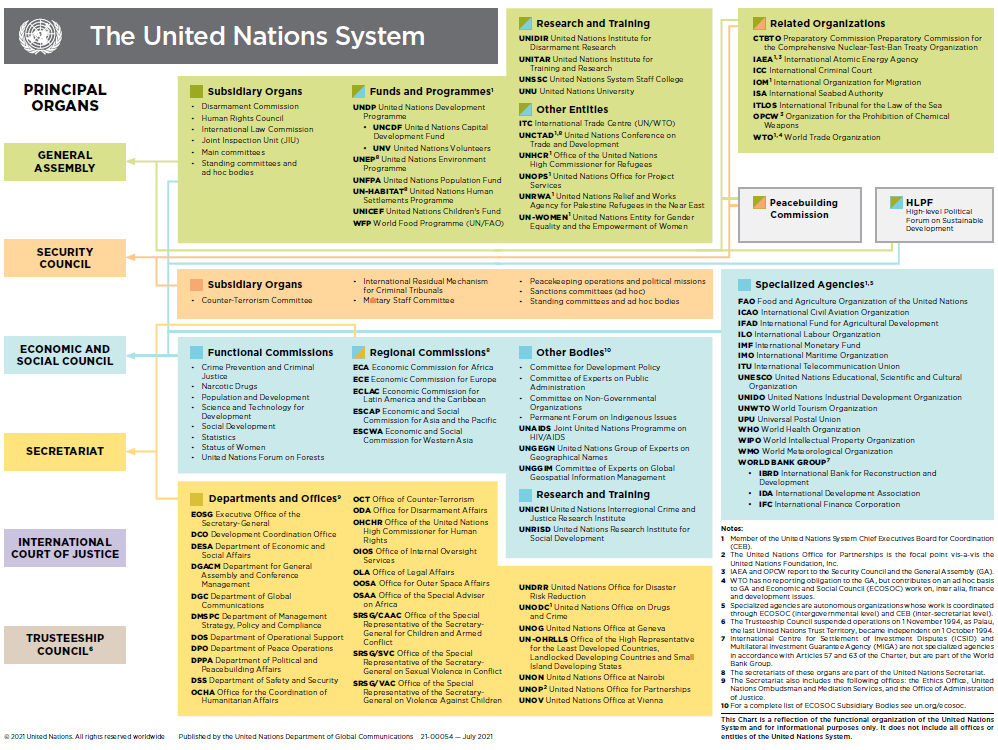
\includegraphics[width=\textwidth,height=\textheight,keepaspectratio]{UNorg.png}
	\end{figure}
\end{frame}	

\begin{frame} 
	\frametitle{\LARGE{UN Institutional Structure}}
	\begin{itemize}
		\item \textbf{General Assembly}: All UN members have one vote, generally on budgets for specialized UN agencies with specific missions.
		\item \textbf{UN Security Council}: 5 permanent members (``P5") and 10 rotating members with 2-year terms.
		\begin{itemize}
			\item P5: US, UK, France, Russia, (People's Republic of) China. \pause
			\item Every member of the P5 has veto power over any resolution. \pause
			\item By majority vote, the UNSC decides if international aggression has happened and how to respond to it. 			
		\end{itemize}
	\end{itemize}
\end{frame}

\begin{frame} 
	\frametitle{\LARGE{UNSC and Security Outcomes}}
	\begin{itemize}
		\item What does the structure of the UNSC imply? \pause That the P5 will use their veto to defend themselves and their client states from actions they don't like. \pause
		\item Examples:
		\begin{itemize}
			\item Russia has blocked several resolutions condemning the killing of civilians in the Syrian civil war. \pause
			\item US has blocked several resolutions condemning the killing of civilians in the Israeli-Palestinian conflict. \pause
		\end{itemize}
	\item This general phenomenon is called \textbf{policy bias}. 
	\end{itemize}
\end{frame}

\begin{frame} 
	\frametitle{\LARGE{Types of UNSC Actions}}
	\begin{itemize}
		\item \textbf{Peace enforcement}: intervention in an active conflict to force an aggressor to stop. This authorizes the use of force against the aggressor by the international community. \pause
		\begin{itemize}
			\item Only three examples: Korean War, Gulf War, 2011 NATO intervention in Libya. \pause
		\end{itemize}
		\item \textbf{Peacekeeping}: resolves commitment problems between two potential opponents by providing impartial monitors for a disputed area, ceasefire, transition to elections, etc. \pause
		\begin{itemize}
			\item These monitors raise the costs of aggression not only by informing potential targets but also because an aggressor usually needs to harm neutral peacekeepers in order to get to their opponent. \pause
		\end{itemize}
	\end{itemize}
\end{frame}

%from https://peacekeeping.un.org/en/where-we-operate fact sheet
\begin{frame} 
	\frametitle{\LARGE{2023 Active Peacekeeping Missions}}
	\begin{figure}[ht!]
		\centering
		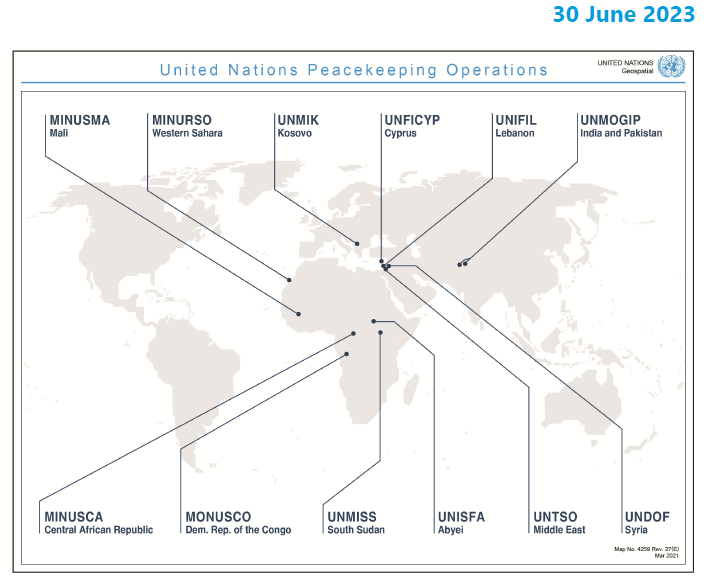
\includegraphics[width=\textwidth,height=\textheight,keepaspectratio]{UNpeacekeeping.png}
	\end{figure}
\end{frame}	

\begin{frame} 
	\frametitle{\LARGE{Collective Security: A Success Story?}}
	\begin{itemize}
		\item By their nature, successful collective security actions tend to be ``quiet:" stories of international harmony, successful rebuilding, etc. tend to get less coverage than disasters. \pause
		\item On average, UN peacekeeping has been quite successful.
		\begin{itemize}
			\item Examples: El Salvador, Guatemala, Mozambique, Cambodia
			\item These successes frequently involve disarming rebel groups, integrating former rebels into society, and organizing elections to help political system recover.
		\end{itemize}
	\end{itemize}
\end{frame}

\begin{frame} 
	\frametitle{\LARGE{Collective Security: A Success Story?}}
	\begin{itemize}
		\item UN peace enforcement is a different story. \pause
		\item The UN only imperfectly deals with the collective action problems surrounding peace enforcement. \pause
		\item Most obvious failure to engage in peace enforcement is the Rwandan Genocide. \pause
		\item 1992 breakup of the former Yugoslavia was another failure, as a UN peacekeeping force was unable to prevent Serbian massacres of Bosnian Muslims. NATO intervention eventually ended the conflict.
	\end{itemize}
\end{frame}

\begin{frame} 
	\frametitle{\LARGE{Summary}}
	\begin{itemize}
		\item Institutions such as NATO can be a source of peace through credible deterrence. \pause
		\item The UN is most successful when strong states agree, and when at least one strong state takes an interest in the conflict and is willing to pay costs. \pause
		\item While the UN has limits, is it better than nothing?		
	\end{itemize}
\end{frame}

\begin{frame} 
	\frametitle{\LARGE{Central Question 2}}
	\centering
	\Large{What conflict research has been published recently at UNC?}
\end{frame}

\begin{frame} 
	\frametitle{\LARGE{Key Terms}}
	\begin{itemize}
		\item Market power politics
		\item Strategic delay
		\item Grey zone tactics
		\item Salami expansion
		\item Petrodollar system
	\end{itemize}
\end{frame}

\begin{frame} 
	\frametitle{\LARGE{Market Power Politics}}
	\begin{itemize}
		\item This chapter (and the rest of the book) is concerned with how and when states engage in territorial expansionist behaviors. \pause
		\item \textbf{Market power politics theory argues that competition for market power gives states incentives to expand their territory or prevent other states from expanding.}
		\item However, since WWII, a norm of international respect for settled borders has (generally) prevailed. \pause
		\item This leads to constraints on a state's actions. 
	\end{itemize}
\end{frame}

\begin{frame} 
	\frametitle{\LARGE{Constraints}}
	\begin{itemize}
		\item If a state's goal is to expand its market power by expanding its territorial control, what might constrain its actions? Two factors: \pause
		\item \textbf{Economic interdependence}: sufficient dependence on a globalized economy, which would be disrupted by open conflict, can dissuade states from open conflict. \pause
		\item \textbf{International institutions}: states may anticipate that the dispute resolution mechanisms would lead to an outcome that would be suboptimal from a domestic political standpoint.
	\end{itemize}
\end{frame}	

\begin{frame} 
	\frametitle{\LARGE{Constraints}}
	\begin{itemize}
		\item In situations of extremely low constraints, states may simply go to war to grab economically desirable territory. \pause
		\item In situations of extremely high constraints, states will be forced to accept peaceful settlements, even if they are suboptimal. \pause
		\item This theory is most concerned with situations where there is a mixture of high and low constraints. \pause 
		\item In these cases, states can use a tactic of \textbf{strategic delay}.
	\end{itemize}
\end{frame}	

\begin{frame} 
	\frametitle{\LARGE{Strategic Delay}}
	\begin{itemize}
		\item \textbf{Strategic delay}: purposeful postponement of a violent or non-violent settlement of a dispute  with the goal of trying to achieve a more preferable outcome in the future. \pause
		\item This delaying tactic gives states time to implement \textbf{gray zone tactics}: not the overt use of military force, but also not behavior traditionally accepted within international diplomacy. \pause
		\begin{itemize}
			\item These tactics let states slowly pursue their territorial claims over time, while avoiding major armed conflict. \pause
		\end{itemize}	
		\item Grey zone tactics frequently involve \textbf{salami expansion}: small, cumulative steps each of which is too minor to fight over, but at their culmination leads to an outcome that would have triggered conflict if carried out all at once. 
	\end{itemize}
\end{frame}

\begin{frame} 
	\frametitle{\LARGE{The End Goal}}
	\begin{itemize}
		\item The overarching goal of states engaging in this behavior is to use this expanded territorial control to increase a state's \textbf{market power}, allowing it to extract higher profits (``rents"), especially if an industry is state-controlled. \pause
		\item This is desirable for several reasons:
		\begin{itemize}
			\item Increased state revenue
			\item Domestic political stability (if resource is vital for daily life)
			\item International bargaining power
		\end{itemize}
		\item This theory focuses on ``hard commodities," which are natural resources like oil, gas, or rare minerals.	
	\end{itemize}
\end{frame}

\begin{frame} 
	\frametitle{\LARGE{Petrodollar System}}
	\begin{itemize}
		\item \textbf{Petrodollar system}: the sale of petroleum in US dollars. \pause
		\item The majority of petroleum and related products are sold in USD. \pause
		\item Why? One consequence of the US going off the gold standard in the 1970s. 
	\end{itemize}
\end{frame}

\begin{frame} 
	\frametitle{\LARGE{Formal Model}}
	\begin{itemize}
		\item If the host state is participating in the petrodollar system by producing and exporting oil, this helps America's economy by keeping the dollar valuable. \pause
		\item Given the economic benefits of a strong dollar, this means the US has rational incentives to protect such an economic system. \pause
		\item This can involve the US sending military aid to oil producers (``host states") to ensure their security, as a destabilized or failed state will no longer participate in the global petrodollar system.
	\end{itemize}
\end{frame}

\begin{frame} 
	\frametitle{\LARGE{Formal Model: Moral Hazards}}
	\begin{itemize}
		\item Say that host state has a terrorist problem. \pause
		\item If it receives military aid to increase its security, this decreases its incentives to bargain with or eliminate the terrorists. Why? \pause
		\begin{itemize}
			\item \textbf{If the terrorism stops, so does the flow of aid.}
		\end{itemize}
		\item This aid strengthens the government such that its leaders are able to stay in power (particularistic benefits), while the costs of an ongoing terrorism campaign are borne by the general population.
	\end{itemize}
\end{frame}

\begin{frame} 
	\frametitle{\LARGE{Formal Model: Moral Hazards}}
	\begin{itemize}
		\item This incentive structure is especially helpful to the host state if it is engaging in the kinds of corruption and human rights abuses that normally lead to aid being suspended. \pause
		\item In response to any threatened decrease in aid, the host state can argue that it is in America's economic interest to keep the state functional, as this way its participation in the petrodollar system continues. 
	\end{itemize}
\end{frame}

\begin{frame} 
	\frametitle{\LARGE{Formal Model: The Take-Away}}
	\begin{itemize}
		\item US military aid for fighting terrorism does not actually decrease the amount of terrorism, but instead prolongs it, while also serving US interests in stability of the petrodollar system.
	\end{itemize}
\end{frame}


\end{document}
